\documentclass[13pt,oneside]{book}
\usepackage[utf8]{inputenc}
\usepackage{url}
\usepackage{listings}
\usepackage{graphicx}

\usepackage{geometry}
\geometry{a4paper, left=20mm, right=20mm, top=20mm, bottom=20mm}
\usepackage[margin=1.2in]{geometry}
\usepackage[toc,page]{appendix}
\usepackage{graphicx}
\usepackage{natbib}
\usepackage{lipsum}
\usepackage{caption}

\begin{document}

\captionsetup[figure]{margin=1.5cm,font=small,labelfont={bf},name={Figure},labelsep=colon,textfont={it}}
\captionsetup[table]{margin=1.5cm,font=small,labelfont={bf},name={Table},labelsep=colon,textfont={it}}
\setlipsumdefault{1}

\begin{titlepage}
\begin{center}
{\LARGE College Of Engineering Trivandrum}\\[3cm]
\linespread{1.2}\huge {\bfseries System Software Lab}\\[3cm]
\linespread{1}

\includegraphics[width=5cm]{img/emblem.jpeg}\\[3cm]
{\Large GOKUL K\\ S5  CSE \\ Roll No:21\\ TVE18CS021 }\\[1cm]


\textit{ }\\[2cm]
Department of Computer Science\\[0.2cm]
\today
\end{center}

\end{titlepage}

\newpage

\begin{frame}{}
    \centering
    \hspace*{-0.5cm}
    $\vcenter{\hbox{
\includegraphics[width=1.5cm]{img/emblem.jpeg}}}$
    $\vcenter{\resizebox{0.95\textwidth}{!}{
        \begin{tabular}{c}
             CS331 - System Software Lab $\cdot$ 2020 $\cdot$   \\
             \hline 
        \end{tabular}
    }}$
\end{frame}
\section*{Cycle 2}
\section*{Expt 9}
\begin{center}
    \Large{Pass 2 of a two pass assembler}
\end{center}
\section*{Aim}
\large
Implement pass two of a two pass assembler

\section*{Algorithm} 
    \begin{verbatim}
1 begin
2 read first input file { from intermediate file }
3 if OPCODE = ’START ’ then
4 begin
5 write listing line
6 read next input line
7 end {if START }
8 write header record to object program
9 initialized first Text record
10 while OPCODE != ’END ’ do
11 begin
12 if this is not a comment line then
13 begin
14 search OPTAB for OPCODE
15 if found then
16 begin
17 if there is a symbol in OPERAND field then
18 begin
19 search SYMTAB for OPERAND
20 if found then
21 store symbol value as operand address
22 else
23 begin
24 store 0 as operand address
25 set error flag ( undefined symbol )
26 end
27 end {if symbol }
28 else
29 store 0 as operand address
30 assemble the object code instruction
31 end {if opcode found }
32 else if OPCODE = ’BYTE ’ or ’WORD ’ then
33 convert constant to object code
34 if object code not fit into the current Text record then
35 begin
36 write Text record to object program
37 initialized new Text record
38 end
39 add object code to Text record
40 end {if not comment }
41 write listing line
42 read next input line
43 end { while not END }
	\end{verbatim}

\section*{Source Code}
\small

\begin{lstlisting}[language=C]
/* 
  Pass 2 of a Two Pass Assembler
*/

#include <stdio.h>
#include <stdlib.h>
#include <string.h>

void display();

char *my_itoa(int num, char *str)
{
        if(str == NULL)
        {
                return NULL;
        }
        sprintf(str, "%d", num);
        return str;
}

int main()
{
    char a[10], ad[10], label[10], opcode[10], operand[10], symbol[10];
    int start, diff, i, address, add, len, actual_len, finaddr, prevaddr, j = 0;
    char mnemonic[15][15] = {"LDA", "STA", "LDCH", "STCH"};
    char code[15][15] = {"33", "44", "53", "57"};

    FILE *fp1, *fp2, *fp3, *fp4;
    fp1 = fopen("output.txt", "w");
    fp2 = fopen("symtab.txt", "r");
    fp3 = fopen("intermediate.txt", "r");
    fp4 = fopen("objcode.txt", "w");

    fscanf(fp3, "%s\t%s\t%s", label, opcode, operand);

    while (strcmp(opcode, "END") != 0)
    {
        prevaddr = address;
        fscanf(fp3, "%d%s%s%s", &address, label, opcode, operand);
    }
    finaddr = address;
    
    fclose(fp3);
    fp3 = fopen("intermediate.txt", "r");

    fscanf(fp3, "\t%s\t%s\t%s", label, opcode, operand);
    if (strcmp(opcode, "START") == 0)
    {
        fprintf(fp1, "\t%s\t%s\t%s\n", label, opcode, operand);
        fprintf(fp4, "H^%s^00%s^00%d\n", label, operand, finaddr);
        fscanf(fp3, "%d%s%s%s", &address, label, opcode, operand);
        start = address;
        diff = prevaddr - start;
        fprintf(fp4, "T^00%d^%d", address, diff);
    }

    while (strcmp(opcode, "END") != 0)
    {
        if (strcmp(opcode, "BYTE") == 0)
        {
            fprintf(fp1, "%d\t%s\t%s\t%s\t", address, label, opcode, operand);
            len = strlen(operand);
            actual_len = len - 3;
            fprintf(fp4, "^");
            for (i = 2; i < (actual_len + 2); i++)
            {   
                // itoa(operand[i], ad, 16);
                sprintf(ad,"%x",operand[i]);
                fprintf(fp1, "%s", ad);
                fprintf(fp4, "%s", ad);
            }
            fprintf(fp1, "\n");
        }

        else if (strcmp(opcode, "WORD") == 0)
        {
            len = strlen(operand);
            // itoa(atoi(operand), a, 10);
            sprintf(a,"%d",atoi(operand));
            fprintf(fp1, "%d\t%s\t%s\t%s\t00000%s\n", address, label, opcode, operand, a);
            fprintf(fp4, "^00000%s", a);
        }

        else if ((strcmp(opcode, "RESB") == 0) || (strcmp(opcode, "RESW") == 0)) {
            fprintf(fp1, "%d\t%s\t%s\t%s\n", address, label, opcode, operand);
        }

        else
        {
            while (strcmp(opcode, mnemonic[j]) != 0)
                j++;
            if (strcmp(operand, "COPY") == 0)
                fprintf(fp1, "%d\t%s\t%s\t%s\t%s0000\n", address, label, opcode, operand, code[j]);
            else
            {
                rewind(fp2);
                fscanf(fp2, "%s%d", symbol, &add);
                while (strcmp(operand, symbol) != 0)
                    fscanf(fp2, "%s%d", symbol, &add);
                fprintf(fp1, "%d\t%s\t%s\t%s\t%s%d\n", address, label, opcode, operand, code[j], add);
                fprintf(fp4, "^%s%d", code[j], add);
            }
        }

        fscanf(fp3, "%d%s%s%s", &address, label, opcode, operand);
    }

    fprintf(fp1, "%d\t%s\t%s\t%s\n", address, label, opcode, operand);
    fprintf(fp4, "\nE^00%d", start);
    
    fclose(fp4);
    fclose(fp3);
    fclose(fp2);
    fclose(fp1);

    display();
    printf("\n");
    return 0;
}

void display() {
    char ch;
    FILE *fp1, *fp2, *fp3, *fp4;

    printf("\nIntermediate file is converted into object code");

    printf("\n\nThe contents of Intermediate file:\n\n");
    fp3 = fopen("intermediate.txt", "r");
    ch = fgetc(fp3);
    while (ch != EOF)
    {
        printf("%c", ch);
        ch = fgetc(fp3);
    }
    fclose(fp3);

    printf("\n\nThe contents of Symbol Table :\n\n");
    fp2 = fopen("symtab.txt", "r");
    ch = fgetc(fp2);
    while (ch != EOF)
    {
        printf("%c", ch);
        ch = fgetc(fp2);
    }
    fclose(fp2);

    printf("\n\nThe contents of Output file :\n\n");
    fp1 = fopen("output.txt", "r");
    ch = fgetc(fp1);
    while (ch != EOF)
    {
        printf("%c", ch);
        ch = fgetc(fp1);
    }
    fclose(fp1);

    printf("\n\nThe contents of Object code file :\n\n");
    fp4 = fopen("objcode.txt", "r");
    ch = fgetc(fp4);
    while (ch != EOF)
    {
        printf("%c", ch);
        ch = fgetc(fp4);
    }
    fclose(fp4);

}
    \end{lstlisting}
    \begin{verbatim}
input.txt

COPY START 1000
** LDA ALPHA
** ADD ONE
** SUB TWO
** STA BETA
ALPHA BYTE C'KLNCE
ONE RESB 2
TWO WORD 5
BETA RESW 1
** END **
    
optab.txt
LDA 00
STA 23
ADD 01
SUB 05
    \end{verbatim}
    \section*{Output}
    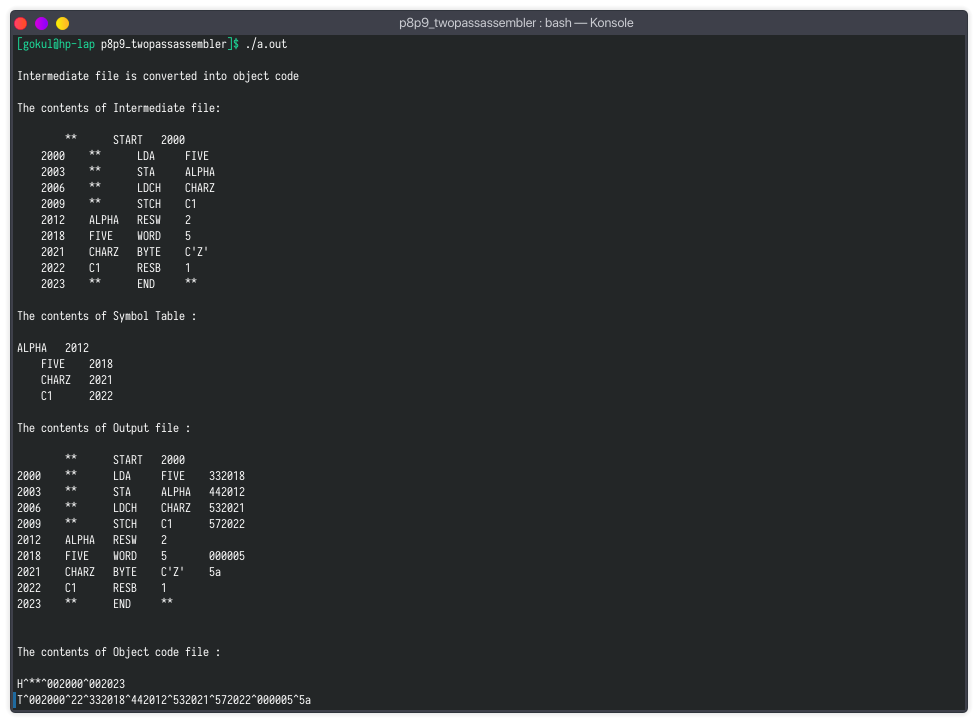
\includegraphics[width=\textwidth]{img/p9.png}
    
\Large
\section*{Result}
\large
The pass two of a two pass assembler was implemented and its output verified
\end{document}